
\documentclass[a4paper,14pt]{extarticle}
\usepackage[utf8]{inputenc}
\usepackage[english,russian]{babel}

\usepackage{tikz}

\usepackage{setspace}
\singlespacing % одинарный интервал

\usepackage{amsmath}
\usepackage{amsfonts}
\usepackage{amssymb}
\usepackage{mathtext}
\usepackage{graphicx}
\usepackage{float}
\usepackage[left=3cm, right=1cm, top=1.5cm, bottom=1.5cm]{geometry}
\usepackage{icomma} % "Умная" запятая: $0,2$ --- число, $0, 2$ --- перечисление
\usepackage{indentfirst} % Красная строка.

\usepackage{minted}

\renewcommand{\thesection}{\arabic{section}}

\begin{document}
\begin{titlepage}
  \begin{center}
    ГОУ ВО АЛТАЙСКИЙ ГОСУДАРСТВЕННЫЙ УНИВЕРСИТЕТ
    \vspace{0.25cm}
    
    Физико-технический факультет
    
    Кафедра вычислительной техники и электроники
    \vfill
    
    {\LARGE Виртуализация ОС}\\[5mm]
    \textsc{(Отчёт по индивидуальному заданию по курсу <<Операционные системы>>)}
  \bigskip

\end{center}
\vfill

\newlength{\ML}
\settowidth{\ML}{«\underline{\hspace{0.7cm}}» \underline{\hspace{2cm}}}
\hfill\begin{minipage}{0.4\textwidth}
  Выполнил студент 2-го курса, 585 группы:\\
  \underline{\hspace{\ML}} А.\,К.~Роженцев\\
  «\underline{\hspace{0.7cm}}» \underline{\hspace{2cm}} \the\year~г.
\end{minipage}%
\bigskip

\hfill\begin{minipage}{0.4\textwidth}
  Проверил\\
  \underline{\hspace{\ML}} П.\,Н.~Уланов\\
  «\underline{\hspace{0.7cm}}» \underline{\hspace{2cm}} \the\year~г.
\end{minipage}%
\vfill

\begin{center}
  Барнаул, \the\year~г.
\end{center}
\end{titlepage}

%\maketitle

\tableofcontents

\section{Введение и постановка задачи}
1. Познакомиться с гипервизорами Hyper-V, KVM, VirtualBox, Xen;
\newline
2. Создать виртуальную машину и произвести установку <<гостевой>> системы;
\newline
3. Произвести настройку гостевой системы.
\newline
\section{ Hyper-V, KVM, VirtualBox, Xen}


\centering
Microsoft Hyper-V — система аппаратной виртуализации для x64-систем на основе гипервизора. Бета-версия Hyper-V была включена в x64-версии Windows Server 2008, а законченная версия была выпущена 26 июня 2008. Ранее была известна как виртуализация Windows Server. 
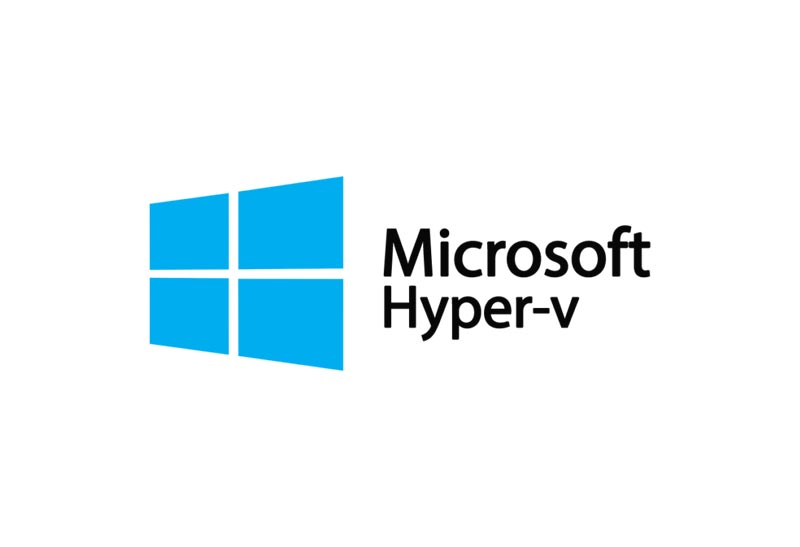
\includegraphics[width=0.9\linewidth]{Microsoft_Hyper_V.jpg}
\caption{Hyper-V}
\label{fig:mpr}



\centering
KVM — программное решение, обеспечивающее виртуализацию в среде Linux на платформе x86, которая поддерживает аппаратную виртуализацию на базе Intel VT либо AMD SVM.
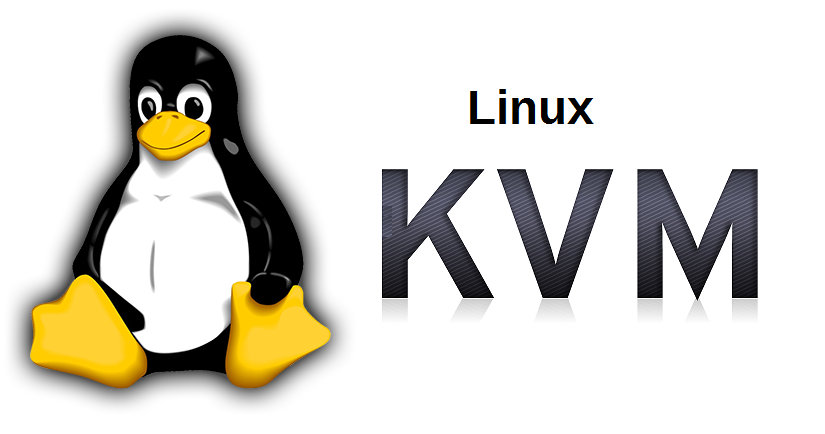
\includegraphics[width=0.75\linewidth]{linux-kvm.png}
\caption{KVM}
\label{fig:mpr}




\centering
VirtualBox — программный продукт виртуализации для операционных систем Microsoft Windows, Linux, FreeBSD, macOS, Solaris/OpenSolaris, ReactOS, DOS и других.

\includegraphics[width=0.9\linewidth]{Virtualbox_logo.png}
\caption{VirtualBox}
\label{fig:mpr}





\centering
Xen — кроссплатформенный гипервизор, разработанный в компьютерной лаборатории Кембриджского университета и распространяемый на условиях лицензии GPL.

\includegraphics[width=1\linewidth]{Xen_hypervisor_logo_black.svg.png}
\caption{Xen}
\label{fig:mpr}


\newpage
\section{Установка и настройка виртуальной машины}



\centering
Установка Debian 10.4.0 Gnome на примере гипервизора VirtualBox
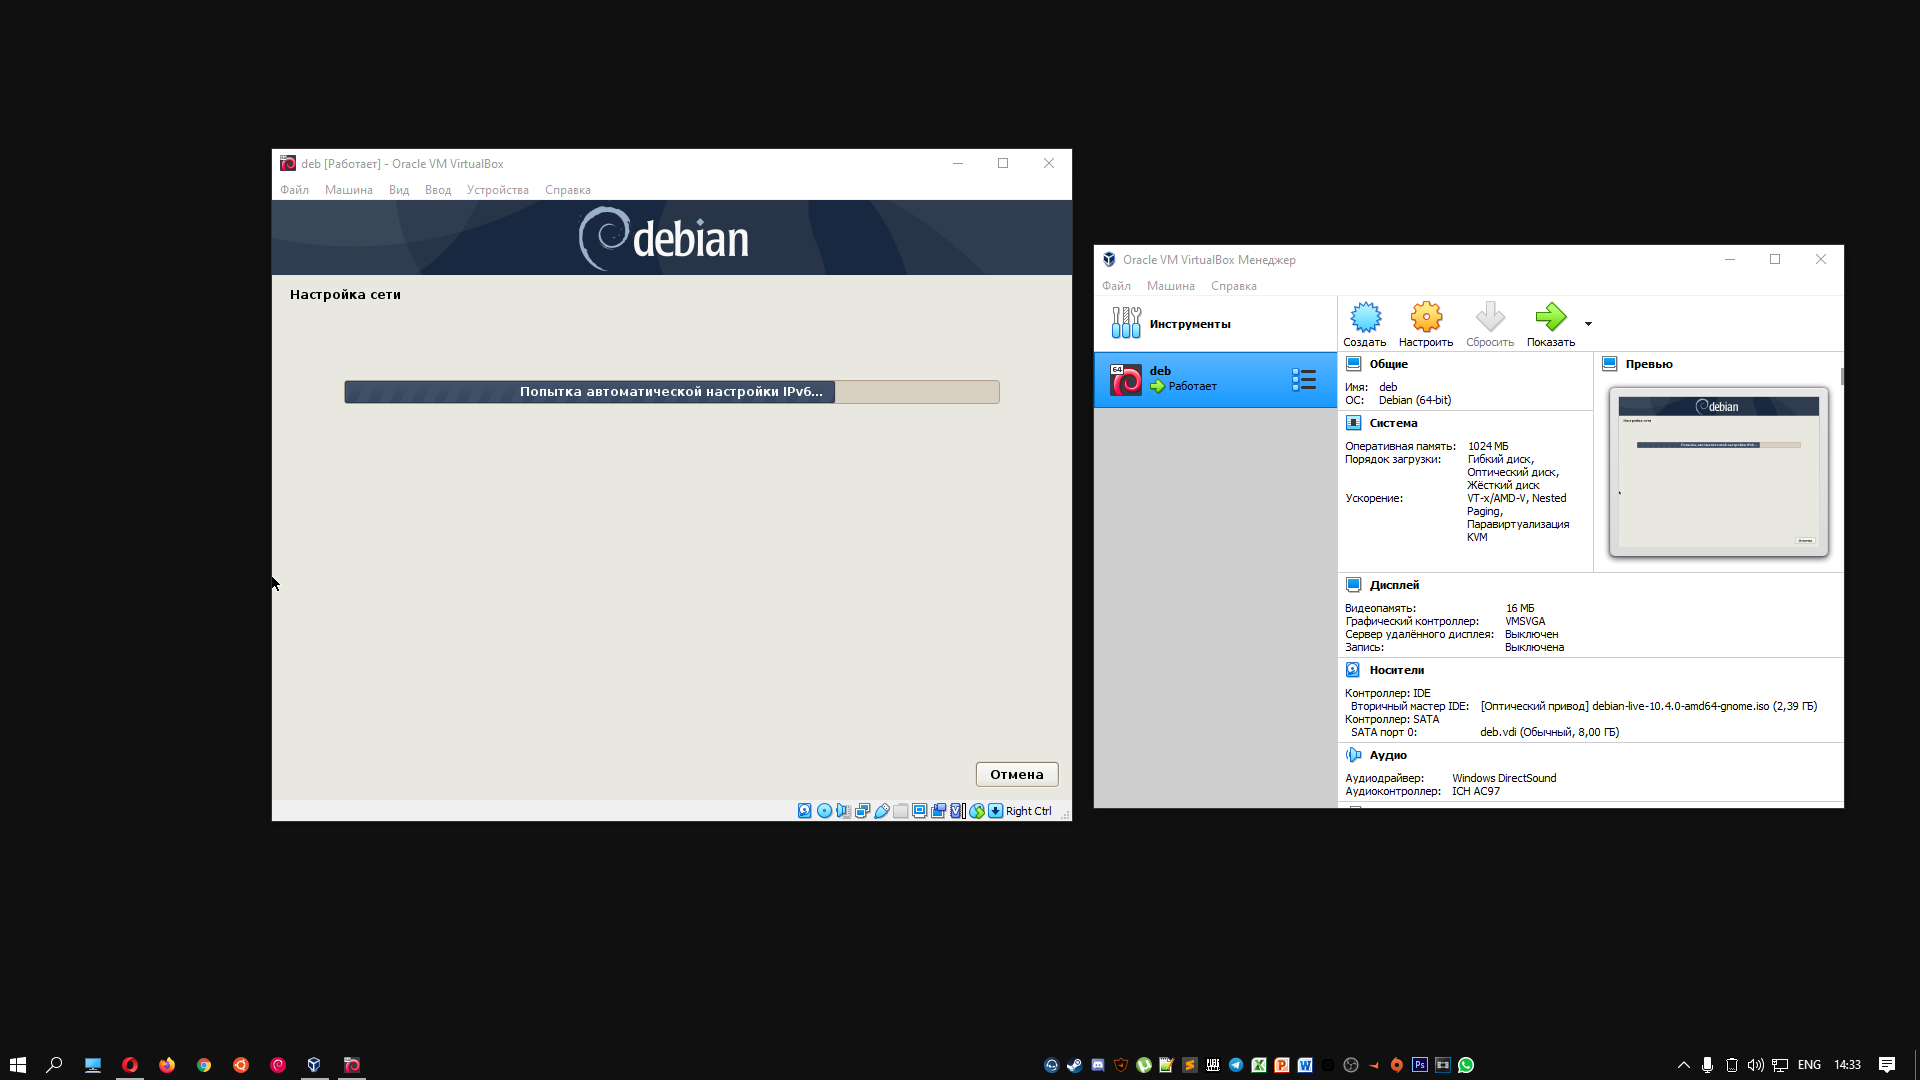
\includegraphics[width=1\linewidth]{install.png}
\caption{Install}
\label{fig:mpr}




\centering
Настойка виртуальной машины.
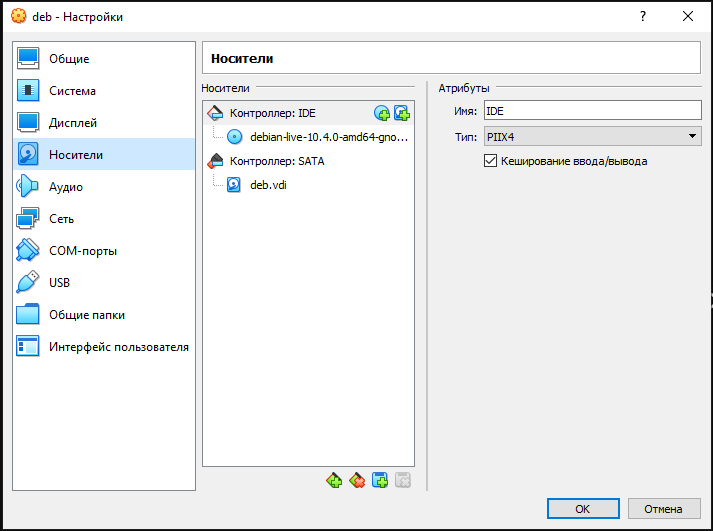
\includegraphics[width=1\linewidth]{settings.png}
\caption{settings}
\label{fig:mpr}




\centering
Сеть после настройки виртуальной машины.
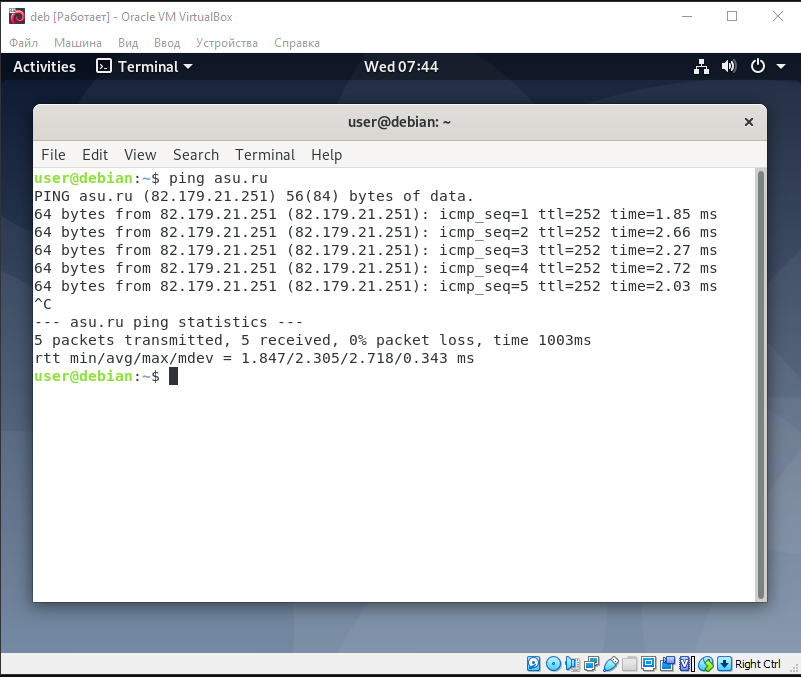
\includegraphics[width=1\linewidth]{work.png}
\caption{ping asu.ru}
\label{fig:mpr}




\newpage

\section{Вывод}

Была установлена вирутальная машина с системой Debian 10.4.0 Gnome, и произведена настройка.
Вполне удобная рабочая система, за исключением низкой скорости работы по причине малого выделения ресурсов основной системой. Из плюсов можно выделить наличие возможноси ставить абсолютно любую систему и даже несколько. Из минусов, опять же - скорость работы.

\end{document} 

